\documentclass[11pt,letterpaper]{article}
\usepackage[T1]{fontenc}
\usepackage[utf8]{inputenc}
\usepackage{lmodern,microtype}
\usepackage[margin=0.92in,headheight=15pt]{geometry}
\usepackage{amsmath,amssymb,amsthm,mathtools,bm}
\usepackage{booktabs,array,tabularx,longtable}
\usepackage{graphicx,xcolor}
\usepackage[font=small,labelfont=bf]{caption}
\usepackage{enumitem,needspace,fancyhdr}
\usepackage[numbers,sort&compress]{natbib}
\usepackage[most]{tcolorbox}
\usepackage[colorlinks=true,linkcolor=blue!45!black,citecolor=blue!45!black,
urlcolor=blue!45!black,pdftitle={Selective Overlap Records},
pdfsubject={Preserving task information through ordered neural transitions}]{hyperref}
\definecolor{ink}{HTML}{19374D}
\definecolor{teal}{HTML}{116B70}
\definecolor{light}{HTML}{EDF7F6}
\definecolor{muted}{HTML}{586975}
\setlength{\parindent}{0pt}
\setlength{\parskip}{5.5pt}
\setlength{\emergencystretch}{3em}
\setlist{nosep,leftmargin=1.4em}
\widowpenalty=10000
\clubpenalty=10000
\allowdisplaybreaks[1]
\setcounter{tocdepth}{1}
\pagestyle{fancy}
\fancyhf{}
\fancyhead[L]{\small\color{ink}Selective Overlap Records}
\fancyhead[R]{\small\color{muted}Research proposal}
\fancyfoot[L]{\scriptsize\color{muted}Working draft 1.0}
\fancyfoot[R]{\small\thepage}
\newtcolorbox{keybox}{colback=light,colframe=teal,boxrule=0.6pt,
arc=2pt,left=9pt,right=9pt,top=7pt,bottom=7pt,breakable}
\newtheorem{theorem}{Theorem}[section]
\newtheorem{proposition}[theorem]{Proposition}
\newtheorem{lemma}[theorem]{Lemma}
\newtheorem{corollary}[theorem]{Corollary}
\theoremstyle{definition}
\newtheorem{definition}[theorem]{Definition}
\theoremstyle{remark}
\newtheorem{remark}[theorem]{Remark}
\newcommand{\R}{\mathbb R}
\newcommand{\E}{\mathbb E}
\newcommand{\Var}{\operatorname{Var}}
\newcommand{\rank}{\operatorname{rank}}
\newcommand{\row}{\operatorname{row}}
\newcommand{\im}{\operatorname{im}}
\newcommand{\diag}{\operatorname{diag}}
\newcommand{\ReLU}{\operatorname{ReLU}}
\newcommand{\CReLU}{\operatorname{CReLU}}
\newcommand{\norm}[1]{\left\lVert#1\right\rVert}
\newcommand{\inner}[2]{\left\langle#1,#2\right\rangle}
\newcommand{\pos}[1]{\left[#1\right]_+}
\newcommand{\code}[1]{\texttt{\detokenize{#1}}}
\begin{document}
\thispagestyle{plain}
{\color{teal}\small RESEARCH PROPOSAL \quad / \quad 25 OCTOBER 2026}
\vspace{8pt}

{\LARGE\bfseries\color{ink}Selective Overlap Records\par}
\vspace{4pt}
{\large Preserving task information through ordered neural transitions\\
and reconstructing it with atlas gluing\par}
\vspace{10pt}
{\small Working draft 1.0. Mathematical derivations, implementation proposal,
and falsifiable evaluation plan.}
\section{How we got here}
\label{sec:story}

The starting point was a small network that should have been able to solve its
task. The QDO study used an eight-dimensional input and a teacher built from four
orthogonal features, each rectified separately. A four-unit student already had
enough architectural capacity to implement that teacher. Nevertheless, some
training runs converged to representations that merged distinctions the answer
still depended on. The failure was visible inside the computation: different
inputs could reach the same complete intermediate state while requiring different
outputs \cite{qdo,projection}.

One especially useful picture was a pair of teacher features \(A\) and \(B\)
whose output coefficients have the same sign. Their input-dependent
preactivations need not share a sign. A failed
representation could keep their common direction, \(A+B\), while weakening their
contrast, \(A-B\). In one diagnosed cohort, geometric retention was about
\(99.6\%\) for the common direction and \(27.7\%\) for the contrast. These are
geometric measurements from that cohort, not percentages of information or of
all model error. The distinction mattered because
\[
  \ReLU(A)+\ReLU(B)\ne\ReLU(A+B)
\]
in general. A positive contribution can disappear when it is first combined with
a negative contribution and only then rectified. The project also certified a
second failure: preactivations that remained different after the linear map
became identical after ReLU \cite{qdo,projection}.

QDO approached the problem through optimization. Its historical anchors lived in
parameter-derived coordinates, and its repulsive update tried to move training
away from configurations already visited. The invariant version removed a
per-neuron scaling ambiguity before measuring those distances. That is a different
intervention from saving an activation contrast. The manuscript reports a
bounded synthetic continuation study; it does not establish a general optimizer
or a guarantee of information preservation. In the present research discussion,
QDO was judged unsuccessful as the direction to pursue and was set aside. This
proposal carries forward the diagnostic lessons, rather than reopening that
optimizer \cite{qdo,discussion}.

The next intuition was deliberately visual. Imagine arbitrary patterns on a
\(9\times9\) grid. Rotate them, place them over one another, and ask what the
result still tells us about the original views. Ordinary addition can make
different patterns indistinguishable. The suggestion was to make overlapping
contributions darker, so that overlap itself leaves a record. The idea quickly
acquired two further requirements: a pile may contain more than two layers, and
the order of the layers matters. Upper layers should receive different, heavier
weights, but those weights must not become another way to erase a lower layer's
contribution.

An early mathematical detour treated the requirement of no lost information as
exact recovery of every original input bit. That led to positional integer
encodings, capacity bounds, and invertible mixtures of known rotations. Those
calculations were useful boundaries: a single ordinary weighted sum cannot
encode arbitrary independent real-valued layers, while known rotations of one
source are a different problem. They also exposed how floating-point rounding
can defeat an algebraic inverse. But complete serialization was a stronger
requirement than the developing proposal needed. These results remain in an
appendix so that the change of objective is explicit.

The decisive clarification brought back the earlier Hodge atlas work. In the
project's description, local charts already have overlaps, transition maps,
consistency conditions, and a reconstruction or gluing step. The question became:
what must survive between two neural slices so that these local descriptions
still determine the target when glued together? A contrast such as \(A-B\) is
one candidate. The required record can be smaller than a complete copy of the
input if every ambiguity it leaves is irrelevant to the required computation
\cite{discussion}.

Recurrent Dragon supplied a related discipline in the research discussion:
respect causal order, distinguish a useful predictive state from a record of the
entire history, and do not infer a preservation guarantee from predictive success.
The present design also keeps actual transition data and nonlinear interactions
available; it does not substitute scalar coalition attributions for them.
Those are design constraints from prior-work discussion, not claims that this
proposal has inherited a previously verified implementation \cite{discussion}.

CReLU then provided a concrete comparison. It retains both positive and negative
parts of a measured response \cite{crelu}. The proposed mechanism asks whether only selected
contrasts or correction quantities need this protection, with atlas reconstruction
aligning them across slices. The proposal is therefore to \emph{capture
target-relevant distinctions before they disappear, preserve their layer and
chart identities, and glue the retained records into a representation whose
remaining ambiguities cannot change the target}.

\begin{keybox}
\textbf{Central claim to establish.}
For a declared target or target family \(T\), the complete retained representation
\(E\) must satisfy
\[
  E(x)=E(x')\quad\Longrightarrow\quad T(x)=T(x').
\]
Overlap compatibility organizes reconstruction. This implication supplies the
information-preservation requirement.
\end{keybox}

\section{Proposal, scope, and evidence}
\label{sec:overview}

The proposed forward computation has an ordinary path and a selective record
path. At a boundary where a projection, merge, activation, or later aggregation
could discard a target-relevant distinction, a small record is emitted from the
information that still exists before that operation. The record carries a layer
index and, when needed, a chart or branch identity. Existing atlas maps relate
records on overlaps. A reconstruction step combines the records with the
ordinary state, and a readout consumes the resulting representation.

\begin{figure}[htbp]
 \centering
 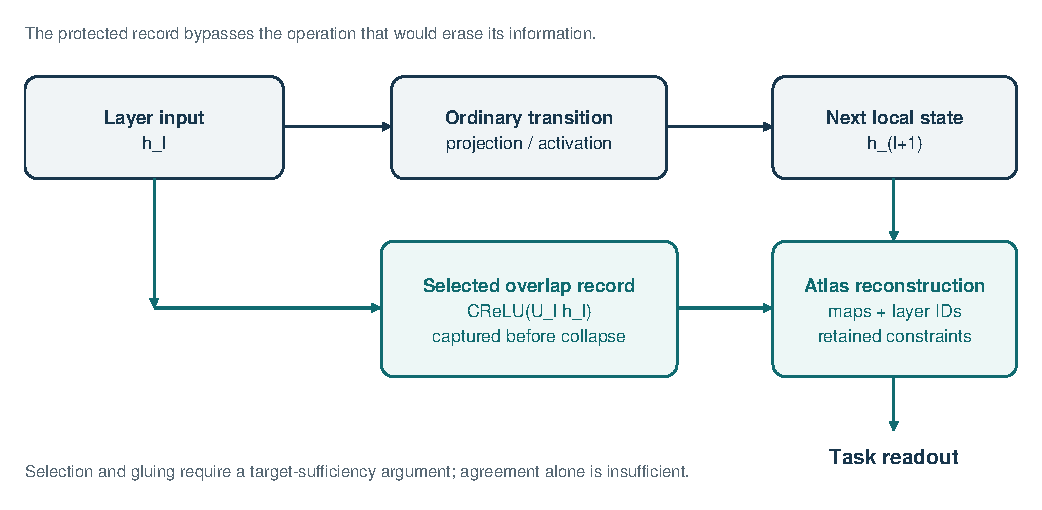
\includegraphics[width=\linewidth]{figures/architecture.pdf}
 \caption{Proposed information path. The record is measured before the
 destructive transition. Its selected coordinates and the reconstruction both
 require a target-sufficiency argument. The diagram does not assume that every
 neural layer is an invertible chart.}
\end{figure}

The main objective is preservation of a declared computation or task family.
Full input reconstruction is a useful reference case, obtained by setting
\(T(x)=x\), but it is not imposed by default. Exact order recovery is a separate
requirement whenever order or source identity must survive independently of the
target value. Such metadata remains explicit.

\begin{center}
\small
\begin{tabularx}{\linewidth}{@{}p{0.27\linewidth}X@{}}
\toprule
Status & What is supported in this proposal\\
\midrule
Proved algebra & Target-factorization criterion; exact ReLU cancellation
correction; finite merge identities; linear target observability; minimal
linear side records; weighted reconstruction and stability bounds.\\
Checked examples & Deterministic finite-domain checks and explicit negative
controls, reproduced by the supplied verification script.\\
Proposed design & Learned selective records, chart transport, record budgets,
and an end-to-end neural readout. These have not been trained here.\\
Not established & A general learning guarantee, lower total compute,
superiority to CReLU or ordinary added capacity, or preservation of every
possible future task.\\
\bottomrule
\end{tabularx}
\end{center}

\paragraph{Provenance.}
QDO and projection-audit statements come from the inspected project manuscript
and report \cite{qdo,projection}. The Hodge atlas mechanism and Recurrent Dragon
lessons are used as described in the research discussion \cite{discussion};
their implementations were not independently re-audited for this proposal.
Public literature supplies comparison points, not evidence that the proposed
neural system already works. The derivations state their assumptions and make
no claim that the elementary identities themselves are new.

\clearpage
\tableofcontents
\newpage

\section{The exact preservation criterion}
\label{sec:sufficiency}

Let \(\mathcal X\) be the allowed source domain and let
\[
 T:\mathcal X\to\mathcal Y
\]
be the target, task-feature vector, or specified collection of downstream
quantities. Let \(E:\mathcal X\to\mathcal E\) include \emph{everything} retained:
ordinary hidden state, side records, layer indices, branch labels, anchors, and
any input-dependent transition metadata.

\begin{theorem}[Target sufficiency]
\label{thm:fibers}
There exists a decoder \(D:E(\mathcal X)\to\mathcal Y\) satisfying
\begin{equation}
 T=D\circ E
 \label{eq:factorization}
\end{equation}
if and only if
\begin{equation}
 E(x)=E(x')\ \Longrightarrow\ T(x)=T(x')
 \qquad\text{for all }x,x'\in\mathcal X.
 \label{eq:fibers}
\end{equation}
\end{theorem}
\begin{proof}
If \(T=D\circ E\), equal encodings have equal decoded targets. Conversely,
for each \(e\in E(\mathcal X)\), choose any \(x\) with \(E(x)=e\) and define
\(D(e)=T(x)\). Condition \eqref{eq:fibers} makes this definition independent
of the chosen preimage.
\end{proof}

The encoder may identify distinct source states, but only when they have the
same required target. Every fiber \(E^{-1}(e)\) must lie inside a target
fiber. Decoder existence is a structural statement; it does not imply that
decoding is cheap, stable, continuous, or learnable from finite data.

For an existing retained state \(h\), if a fiber \(h^{-1}(z)\) contains \(N_z\)
distinct required target values, an added record must have at least \(N_z\)
distinguishable states on that fiber. For a finite digital alphabet, this
requires at least \(\lceil\log_2N_z\rceil\) fixed-width record bits on that
fiber. The needed capacity depends on missing target distinctions, rather
than automatically on every missing input distinction.

\subsection{Task families and unknown future use}

For a family \(\mathcal F\) of future readouts, require
\[
 E(x)=E(x')\Longrightarrow
 f(x)=f(x')\quad\text{for every }f\in\mathcal F.
\]
For a finite family, take \(T=(f_1,\ldots,f_q)\). If every possible source
distinction matters to some allowed future task, the requirement becomes full
injectivity. A selective guarantee therefore needs a declared task family.
Keeping a currently known scalar answer can be much easier than keeping the
computation reusable for other answers.

For a streaming state with unknown future inputs, two histories may be merged
only if every allowed future continuation produces the same required outputs.
Agreement on the current prefix's answer alone does not establish this.

\subsection{The distributional counterpart}

For a deterministic square-integrable scalar target \(Y=T(X)\), the best
squared-error decoder from \(E(X)\) is the conditional mean. Its risk is
\begin{equation}
 R_E=\E\!\left[\Var(Y\mid E(X))\right].
 \label{eq:bayesrisk}
\end{equation}
For any decoder \(\widehat Y=g(E(X))\),
\begin{equation}
 \E[(Y-\widehat Y)^2]
 =R_E+
 \E\!\left[
 \bigl(\E[Y\mid E(X)]-g(E(X))\bigr)^2
 \right].
 \label{eq:bayesdecomp}
\end{equation}
Expand the squared error around the conditional mean. The cross term has
conditional expectation zero, proving the identity.

Thus \(R_E=0\) gives exact target determination almost surely under the source
distribution. It is not a guarantee on inputs outside that support or on
measure-zero exceptions. A finite set of successful reconstructions is weaker.
For intrinsically noisy labels, preserving the complete predictive law
requires preserving the conditional target distribution. If the declared
objective is squared error alone, preserving the conditional mean suffices
to attain the full-information Bayes risk. Zero conditional variance would
instead incorrectly demand removal of irreducible label noise.

\subsection{Sequential preservation}

Let \(s_\ell=(h_\ell,m_\ell)\) be the complete carried state, including earlier
records. A boundary update may have the form
\[
 s_{\ell+1}=G_\ell(s_\ell)
 =\bigl(F_\ell(h_\ell),m_\ell,r_\ell(s_\ell)\bigr).
\]
\begin{proposition}[Composition]
If \(T_0=T\) and, on reachable states, each stage admits \(T_{\ell+1}\) with
\[
 T_\ell=T_{\ell+1}\circ G_\ell,
\]
then
\[
 T=T_L\circ G_{L-1}\circ\cdots\circ G_0.
\]
\end{proposition}
\begin{proof}
Substitute the stage factorizations successively.
\end{proof}

If earlier records are compressed or removed, that operation is another stage
to which the same condition applies. A local record can be sufficient together
with other records without being sufficient by itself. The complete carried
state, rather than an isolated side channel, is the object to audit.

\section{Exact overlap corrections for rectified sums}
\label{loc:section}

The first constructive case turns the overlapping-shadow idea into an exact
local record. A merge can preserve a common component while removing a
contrast that still matters to the target. The proposal is to identify that
missing contribution before the merge and make it available where the
adjacent computation needs it. This formalizes the selective interpretation
developed in the discussion~\cite{discussion}. The results below concern
specified functions and real arithmetic; they do not assume that a learned
selector already knows which features to preserve.

\subsection{Projection loss and rectification loss are different}
\label{loc:two_losses}

Write $\rho(t)=\ReLU(t)=\max(t,0)$. A linear projection $P$ loses every
distinction in its kernel: $P(x+v)=Px$ whenever $Pv=0$. Rectification can then
lose further distinctions because all nonpositive preactivations produce
zero. These are separate operations, with separate requirements for a repair.

The CReLU construction retains the positive and negative parts of a
measurement~\cite{crelu}:
\begin{equation}
 \CReLU(z)=
 \begin{pmatrix}\rho(z)\\\rho(-z)\end{pmatrix},
 \qquad z=\rho(z)-\rho(-z).
 \label{loc:crelu_inverse}
\end{equation}
It therefore preserves the supplied measurement $z$. If $z=Px$, the identity
does not recover a component of $x$ already removed by $P$.

In the motivating pair collapse, let
\begin{equation}
 S=A+B,\qquad D=A-B,\qquad
 H=\rho(S),\qquad F=\rho(A)+\rho(B).
 \label{loc:pair_definition}
\end{equation}
Here $D$ is a contrast lost by the sum. The inputs $(1,-1)$ and $(0,0)$ both
have $S=0$, so even $\CReLU(S)$ gives the same record. Their required targets
are nevertheless $1$ and $0$. This is the distinction identified in the
earlier projection example~\cite{projection}. A record intended to preserve
it must branch before the sum removes it. Merely branching before the
subsequent ReLU is too late.

\subsection{The cancellation correction}
\label{loc:pair_correction}

\begin{proposition}[Exact local correction]
\label{loc:pair_prop}
For every $A,B\in\R$, define
\begin{equation}
 \kappa(A,B)=\rho(A)+\rho(B)-\rho(A+B).
 \label{loc:kappa_definition}
\end{equation}
Then $F=H+\kappa(A,B)$, and the following formulas are equivalent:
\begin{align}
 \kappa(A,B)
 &=\frac{|A|+|B|-|A+B|}{2}
 \label{loc:kappa_absolute}\\
 &=\frac12\rho\bigl(|D|-|S|\bigr)
 \label{loc:kappa_contrast}\\
 &=\begin{cases}
       0,&AB\ge0,\\
       \min(|A|,|B|),&AB<0.
    \end{cases}
 \label{loc:kappa_gate}
\end{align}
In particular, $\kappa$ is nonnegative.
\end{proposition}

\begin{proof}
Use $\rho(t)=(t+|t|)/2$ in \eqref{loc:kappa_definition}. The linear terms
cancel, giving \eqref{loc:kappa_absolute}; the triangle inequality gives
nonnegativity. If $A,B$ have the same sign, $|S|=|A|+|B|\ge|D|$. If their
signs differ, $|D|=|A|+|B|\ge|S|$. Hence
\[
 |A|+|B|=\max(|S|,|D|),
\]
which yields \eqref{loc:kappa_contrast}. In the opposite-sign case,
$|S|=\bigl||A|-|B|\bigr|$, so
\[
 \kappa=\frac{|A|+|B|-\bigl||A|-|B|\bigr|}{2}
        =\min(|A|,|B|).
\]
The same-sign case gives zero, including either input being zero.
\end{proof}

The gate identifies precisely when the collapsed sum loses a contribution
needed by this target. A binary gate alone is insufficient: the missing
amount varies. The record $\kappa$ supplies that amount. Conditional on the
retained value $H$, the transformations $F=H+\kappa$ and $\kappa=F-H$ are
inverse. Thus this record contains exactly the missing target value
conditional on $H$, without specifying which input supplied the positive
contribution or reconstructing the original pair.

Keeping a signed contrast alongside a rectified sum is a different proposal,
and does not suffice in general. The following collision has strictly
negative sums:
\begin{center}
\begin{tabular}{rrrrrr}
\toprule
$A$&$B$&$S$&$H$&$D$&$F$\\
\midrule
$1$&$-4$&$-3$&$0$&$5$&$1$\\
$2$&$-3$&$-1$&$0$&$5$&$2$\\
\bottomrule
\end{tabular}
\end{center}
The retained pair $(H,D)$ is identical while the target differs. Retaining
$(S,D)$ would recover $A=(S+D)/2$ and $B=(S-D)/2$. For this symmetric target,
$(S,|D|)$ also suffices. The correction $(H,\kappa)$ provides a more direct
statement of what the target requires. None of these facts establishes a
computational advantage for one implementation.

The distinction between a gate and a record can also be checked on a whole
family of inputs. Set $(A,B)=(t,-t)$ for $0<t<1$. Every member has $H=0$ and
the same opposite-sign gate, but its target and correction are both $t$.
An exact record must distinguish these target values; a flag saying that
cancellation occurred cannot do so. Conversely, $(t,-t)$ and $(-t,t)$ have
opposite signed contrasts but the same target. This target does not require
the record to distinguish them. The example identifies what must vary in
the record without demanding preservation of an unnecessary distinction.

\subsection{Repairing the original four-feature teacher}
\label{loc:teacher_repair}

In the motivating QDO setup, write the four intrinsic teacher features as
$u_1,\ldots,u_4$. The teacher is~\cite{qdo}
\begin{equation}
 f_\star(x)=
 \frac{-\rho(u_1)+\rho(u_2)-\rho(u_3)+\rho(u_4)}{2}.
 \label{loc:teacher}
\end{equation}
Group the features by their output coefficient sign. Define
\begin{align}
 S_+&=u_2+u_4,&\kappa_+&=\kappa(u_2,u_4),\\
 S_-&=u_1+u_3,&\kappa_-&=\kappa(u_1,u_3).
\end{align}
Applying Proposition~\ref{loc:pair_prop} to each pair gives the exact repair
\begin{equation}
 \boxed{
 f_\star(x)=
 \underbrace{\frac{\rho(S_+)-\rho(S_-)}{2}}_{f_{\rm pair}(x)}
 +\frac{\kappa_+-\kappa_-}{2}.}
 \label{loc:teacher_repair_identity}
\end{equation}
Indeed, the positive pair contributes $\rho(S_+)+\kappa_+$ and the negative
pair contributes $-\rho(S_-)-\kappa_-$. Adding them and dividing by two
reproduces every term of \eqref{loc:teacher}. Each local record is
nonnegative; their contribution to the scalar output has the teacher's
signed coefficients.

This construction identifies sufficient information for the collapsed-pair
example without requiring recovery of all eight ambient input coordinates.
It is an oracle construction when the teacher features $u_j$ are supplied.
A student that has not learned those features cannot calculate these exact
records from an already collapsed representation. Accordingly, an oracle
repair experiment establishes sufficiency of the proposed information;
learning an adequate record remains a separate empirical question. Supplying
the teacher features to a record branch must be disclosed as additional
information in any comparison.

\subsection{Position weights and signed readouts}
\label{loc:weights}

Suppose the required pair target assigns known positive position weights:
\[
 F_\alpha=\alpha_0\rho(A)+\alpha_1\rho(B),
 \qquad 0<\alpha_0<\alpha_1.
\]
The later or upper position receives the larger weight. Positive homogeneity,
$\rho(\alpha A)=\alpha\rho(A)$ for $\alpha>0$, allows the substitutions
$u=\alpha_0A$ and $v=\alpha_1B$. Therefore
\begin{equation}
 F_\alpha=
 \rho(\alpha_0A+\alpha_1B)+\kappa(\alpha_0A,\alpha_1B).
 \label{loc:ordered_pair}
\end{equation}
The common/contrast formulas apply to these weighted inputs. The weights
belong to positions if moving a layer is intended to change its influence.
This target can distinguish some reorderings, but it does not promise to
distinguish every ordering of the original data.

Negative output coefficients require care because
$\rho(\alpha A)=\alpha\rho(A)$ generally fails for $\alpha<0$.
For arbitrary real $\alpha,\beta$, set
\[
 T=\alpha\rho(A)+\beta\rho(B),\qquad S=\alpha A+\beta B.
\]
Expansion of the same ReLU identity yields
\begin{equation}
 T=\rho(S)+R_{\alpha,\beta},\qquad
 R_{\alpha,\beta}
 =\frac{\alpha|A|+\beta|B|-|\alpha A+\beta B|}{2}.
 \label{loc:signed_pair}
\end{equation}
For example, $\alpha=1$, $\beta=-1$, $A=1$, $B=2$ gives $T=-1$, a zero
rectified base, and correction $-1$. A general signed readout therefore
cannot be represented by an unqualified nonnegative correction rule.

\subsection{Arbitrary finite piles and exact local merging}
\label{loc:multiple}

Consider a fixed finite collection $u_1,\ldots,u_K$, where positive
position weights may already have been absorbed into the $u_i$. The required
target is $F_K=\sum_i\rho(u_i)$. Choose any binary merge tree. Each leaf
retains its signed value; each internal node $v$ computes
\[
 S_v=S_{v,L}+S_{v,R},\qquad
 \kappa_v=\kappa(S_{v,L},S_{v,R}).
\]
The child sums must remain signed until this operation has used them.

\begin{theorem}[Telescoping local corrections]
\label{loc:telescoping}
For every such tree,
\begin{equation}
 F_K=\rho(S_{\rm root})+
          \sum_{v\text{ internal}}\kappa_v.
 \label{loc:telescope_equation}
\end{equation}
\end{theorem}
\begin{proof}
Expand each internal record as
$\kappa_v=\rho(S_{v,L})+\rho(S_{v,R})-\rho(S_v)$.
Every nonroot internal node appears once as a child, with a positive term,
and once as a parent, with a negative term. These terms cancel. The remaining
terms are the rectified leaves minus the rectified root, proving the claim.
For one leaf the internal sum is empty and the identity also holds.
\end{proof}

The records need not all remain separate when only this aggregate is needed.
A subtree can carry a signed sum $S$ and accumulated correction $R$. Define
\begin{equation}
 (S_L,R_L)\star(S_R,R_R)=
 \bigl(S_L+S_R,\ R_L+R_R+\kappa(S_L,S_R)\bigr).
 \label{loc:merge_operator}
\end{equation}
Leaves start at $(u_i,0)$. This gives a constant number of scalar fields;
their required numerical range can still grow with the number and weights
of the leaves.

\Needspace{11\baselineskip}
\begin{proposition}[Mass coordinates and the merge law]
\label{loc:mass_coordinates}
Let $P=\sum_i\rho(u_i)$ and $N=\sum_i\rho(-u_i)$. Then
\begin{equation}
 S=P-N,\quad R=\min(P,N),\qquad
 P=\rho(S)+R,\quad N=\rho(-S)+R.
 \label{loc:mass_inverse}
\end{equation}
The merge \eqref{loc:merge_operator} is associative and commutative, with
identity $(0,0)$.
\end{proposition}
\begin{proof}
If $P\ge N$, then $S=P-N\ge0$ and $R=N$, giving both inverse formulas.
If $P<N$, then $S<0$ and $R=P$, again giving them. These formulas establish a
bijection between $(P,N)\in\R_{\ge0}^2$ and $(S,R)\in\R\times\R_{\ge0}$.
Combining two subtrees adds their $P$ and $N$ separately. The resulting
correction is
\begin{align*}
 R_{\rm new}
 &=P_L+P_R-\rho(S_L+S_R)\\
 &=R_L+R_R+\rho(S_L)+\rho(S_R)-\rho(S_L+S_R),
\end{align*}
which is exactly \eqref{loc:merge_operator}. Thus the merge is ordinary
addition in $(P,N)$ coordinates. Associativity, commutativity, and the
identity follow from addition.
\end{proof}

These algebraic properties hold in real arithmetic. Floating-point
implementations can depend on merge order: even the positive leaves
\((10^{16},1,1)\) yield different binary64 sums under the two
parenthesizations.

One immediate consequence connects the correction directly to rectified
sign channels:
\begin{equation}
 \boxed{
 \sum_i\CReLU(u_i)
 =\CReLU\!\left(\sum_i u_i\right)
   +\begin{pmatrix}R\\R\end{pmatrix}.}
 \label{loc:crelu_mass}
\end{equation}
The accumulated positive and negative masses differ from rectifying the
final signed sum by the same cancellation amount in both channels.
The individual seam corrections depend on the merge tree, but their total
$R$ does not.

Commutativity is an explicit limit on the record. The final $(S,R)$ does not
retain the original order: $(1,-1)$ and $(-1,1)$ both yield $(0,1)$. Position
weights can make a specified ordered target respond to a permutation;
source labels and transition direction must remain available when the
subsequent computation requires them. Neither weights nor this two-field
summary guarantee arbitrary future queries. In particular, changing the
readout weights after aggregation can require distinctions no longer
present.

It is useful to distinguish the information needed for the current output
from a state that supports a specified later operation. The pair
$(H,\kappa)$ gives the current target, whereas the merge rule deliberately
carries the signed $S$. For example, the subtree states $(S,R)=(-1,0)$ and
$(-3,0)$ have the same current positive mass, zero, and the same
$(\rho(S),R)$. A later request for $\rho(S+2)$ produces $1$ and $0$,
respectively. The signed sum is necessary for that additional request.
If the only request remains the sum of individually rectified leaves, one
can instead accumulate their positive mass directly. The appropriate state
therefore depends on the operations that will actually follow the overlap.
The explicit $(S,R)$ merge is closed under the signed-sum updates defined
here; its closure does not extend automatically to a new nonlinear readout,
a new set of position weights, or an unspecified future computation.

\paragraph{Signed leaf coefficients.}
For the more general target $\sum_i a_i\rho(A_i)$, initialize
\begin{equation}
 S_i=a_iA_i,\qquad
 R_i=a_i\rho(A_i)-\rho(a_iA_i)
 =\begin{cases}0,&a_i\ge0,\\a_i|A_i|,&a_i<0.\end{cases}
 \label{loc:signed_leaf}
\end{equation}
The negative case follows by writing $a_i=-c$, $c>0$, and using
$\rho(A_i)+\rho(-A_i)=|A_i|$. At every merge,
\[
 \rho(S_L+S_R)+R_{\rm new}
 =\rho(S_L)+R_L+\rho(S_R)+R_R.
\]
Induction therefore recovers the signed target exactly at the root. Here
$R$ may be negative. Omitting the leaf corrections would instead compute
$\sum_i\rho(a_iA_i)$, a different function.

The aggregate considered here can already be computed by directly summing
the rectified leaves. The derivation supplies an exact local accounting
mechanism for a collapsed representation, not evidence of a new efficient
algorithm. Its architectural value must be tested when records are learned
and transported across the actual transitions of interest.

\subsection{Numerical and backward-pass qualifications}
\label{loc:implementation}

The local correction itself has a simple stability property. Let
$\mathcal C=\{(A,B):AB\ge0\}$, the union of the two same-sign quadrants.
Then
\begin{equation}
 \kappa(A,B)=\operatorname{dist}_{\infty}\bigl((A,B),\mathcal C\bigr).
 \label{loc:distance}
\end{equation}
For opposite signs, reaching $\mathcal C$ requires moving at least one
coordinate to zero. Moving the smaller-magnitude coordinate attains
distance $\min(|A|,|B|)$; either coordinate change is a lower bound for
reaching its respective quadrant. Points already in $\mathcal C$ have
distance zero. This proves the identity. Distance to a fixed set is
one-Lipschitz, so perturbing both inputs by at most $\varepsilon$ changes
the ideal correction by at most $\varepsilon$. This is a property of the
function, not a guarantee that every algebraic implementation evaluates it
accurately.

Equivalent real formulas need not behave identically in finite precision.
For $A=-10^{20}$ and $B=1$, the mathematical correction is $1$. In binary64
arithmetic, \eqref{loc:kappa_absolute} can evaluate to zero because the
subtractions lose the small difference. The sign-gated minimum in
\eqref{loc:kappa_gate} returns $1$ for this example. Implement its gate with
sign comparisons rather than the product $AB$, which can overflow. This
avoids a particular subtraction error; signed sums, accumulated records,
and final reconstruction still require numerical error checks.

Forward identities also need a stated backward convention. Differentiating
an exact correction through its source variables gives matching ordinary
derivatives away from activation boundaries. Explicitly, when $A$, $B$, and
$S$ are nonzero,
\begin{equation}
 \frac{\partial\kappa}{\partial A}
 =\mathbf1_{A>0}-\mathbf1_{S>0},\qquad
 \frac{\partial\kappa}{\partial B}
 =\mathbf1_{B>0}-\mathbf1_{S>0}.
 \label{loc:gradient}
\end{equation}
Adding the derivatives of $H$ cancels the common $S$ terms and recovers the
two derivatives of $F$. Thus the exact source-dependent record restores the
derivatives of this specified function as well as its values at these
points. Detaching the record, replacing
it with an approximation, or choosing a different boundary convention can
change training. For example, the exact function
$\rho(z)-\rho(-z)=z$ has derivative one, but automatic differentiation with
$\rho'(0)=0$ on both branches computes zero at $z=0$. The absolute-value
version of the pair correction can also produce a wrong derivative for the
complete target at an internal cancellation boundary. At \(A=1,B=-1\),
using \(|\cdot|'(0)=\rho'(0)=0\) gives the automatic derivative
\((1/2,-1/2)\) for \(H+\kappa\), while the smooth target \(F\) has
gradient \((1,0)\). If preservation of a specified training signal is required,
that signal and its backward convention must be included in the contract
and verified explicitly.

\section{Reconstructing targets from overlapping records}
\label{atl:section}

The atlas idea becomes precise when compatibility and information preservation
are treated as separate requirements. Local records should agree about the
features they share. Their combined information should also determine every
distinction required by the declared target. Agreement alone does not establish
the second property. This section supplies an exact linear model of both
requirements, a construction of minimal selective residuals, and a stability
bound for reconstruction. These are mathematical components proposed for this
architecture; they are not claims that an existing Hodge implementation already
provides the desired neural guarantee.

\subsection{Coordinate charts and partial views}
\label{atl:charts}

A genuine coordinate chart $\phi_i:U_i\to V_i$ is invertible on its domain.
Two charts describing the same underlying object have the transition map
\begin{equation}
  \tau_{ij}=\phi_j\circ\phi_i^{-1}
  \quad\text{on }\phi_i(U_i\cap U_j).
  \label{atl:transition}
\end{equation}
The identities
\begin{equation}
  \tau_{ji}=\tau_{ij}^{-1},
  \qquad
  \tau_{jk}\circ\tau_{ij}=\tau_{ik}
  \label{atl:cocycle}
\end{equation}
hold wherever the compositions are defined; the second identity is evaluated
on the common triple overlap. For affine transitions
$\tau_{ij}(u)=A_{ij}u+b_{ij}$, these conditions imply
\begin{align}
  A_{ji}A_{ij}&=I,
  & b_{ji}&=-A_{ji}b_{ij}, \nonumber\\
  A_{ik}&=A_{jk}A_{ij},
  & b_{ik}&=A_{jk}b_{ij}+b_{jk}.
  \label{atl:affine-cocycle}
\end{align}
The displayed matrix equalities apply when the affine maps agree on overlaps
with nonempty interior in their coordinate spaces. On a smaller constrained
overlap, equality is required only on that overlap.

A many-to-one layer is not automatically such a chart. For partial layer views,
use observation maps $r_i:\mathcal Z\to E_i$ and comparison maps
$\rho_{i,ij}:E_i\to O_{ij}$. The common overlap condition is
\begin{equation}
  \rho_{i,ij}(r_i(z))=\rho_{j,ij}(r_j(z)).
  \label{atl:restriction}
\end{equation}
Neither observation map needs an inverse. Their joint records may still
determine the task. Cellular sheaves provide a standard language for compatible
local data and restriction maps; their degree-zero global sections are
characterized by an agreement operator. The associated spectral theory also
studies reducing edge-message dimensions while preserving global sections
\citep{sheaves}. The proposal uses this organizational idea without assuming
that an arbitrary stack of neural layers is already an atlas or a sheaf with
the required observability properties.

Layer identities, overlap domains, branch choices, and directed transition
maps belong to the retained representation. Ordered composition in
\eqref{atl:cocycle} cannot generally be replaced by an unlabeled weighted sum.

\subsection{The source map and the agreement operator}
\label{atl:two-operators}

Let the source state be $z\in\R^n$, with local records $e_i=M_i z$.
Stack them into $e=Mz\in E=\bigoplus_i E_i$. Let
$\delta:E\to O$ collect overlap discrepancies, for example
$(\delta e)_{ij}=P_{i,ij}e_i-P_{j,ij}e_j$. Correct restrictions satisfy
\begin{equation}
  \delta M=0,
  \qquad\text{hence}\qquad
  \im M\subseteq\ker\delta.
  \label{atl:complex}
\end{equation}
This says that genuine source records agree. The stronger condition
\begin{equation}
  \im M=\ker\delta
  \label{atl:exactness}
\end{equation}
says that every compatible collection has an explanation within the chosen
source model. It is needed for that universal gluing claim, although decoding
records already known to equal $Mz$ does not require it.

The ambiguity left about the source is $\ker M$, not $\ker\delta$.
The latter contains compatible records themselves. In particular,
$\ker(\delta^\top\delta)=\ker\delta$ characterizes agreement; it does not
establish that those records determine the original input or target. If
\eqref{atl:exactness} holds, compatible records identify a source equivalence
class in $\R^n/\ker M$. The remaining question is whether the target is
constant on that class.

\subsection{An exact criterion for target observability}
\label{atl:observability}

Write the required linear task features as $t=Cz\in\R^q$. The rows of $C$
may describe several required readouts. Taking $C=I$ recovers the stronger
requirement of preserving the entire source.

\begin{theorem}[Linear target observability]
\label{atl:observability-theorem}
For unrestricted $z\in\R^n$, the following statements are equivalent:
\begin{enumerate}
  \item Some decoder recovers $Cz$ from $Mz$ for every $z$.
  \item $\ker M\subseteq\ker C$.
  \item $\row(C)\subseteq\row(M)$.
  \item There is a linear matrix $D$ such that $C=DM$.
\end{enumerate}
\end{theorem}

\begin{proof}
If a decoder exists and $v\in\ker M$, then $Mv=M0$, so it must give
$Cv=C0=0$. This proves the second statement. Conversely, that statement says
that two states with the same records have the same target. In finite
dimensional Euclidean spaces, $\row(M)=(\ker M)^\perp$ and likewise for $C$.
Taking orthogonal complements therefore makes the second statement equivalent
to the third. Under the third statement, express each row of $C$ as a linear
combination of rows of $M$ and collect the coefficients into $D$. This gives
$C=DM$. Finally, $D(Mz)=Cz$ provides the required decoder, completing all
implications.
\end{proof}

\begin{corollary}[A well-defined target for every compatible record]
\label{atl:gluing-corollary}
Assume $\im M=\ker\delta$. A linear gluing readout
$\Gamma:\ker\delta\to\R^q$ satisfying $\Gamma(Mz)=Cz$ exists if and only
if $\ker M\subseteq\ker C$. When it exists, one such formula is
$\Gamma(e)=CM^\dagger e$.
\end{corollary}

\begin{proof}
Exactness ensures that every compatible $e$ has a preimage $z$. Any two
preimages differ by a member of $\ker M$. Under the stated kernel inclusion,
they have the same target, so assigning $\Gamma(e)=Cz$ is well-defined.
Preimages can be added and scaled, which makes this assignment linear.
Moreover, $CM^\dagger M=C$ by target observability, proving the formula.
Conversely, the zero record has both $0$ and every $v\in\ker M$ as
preimages. A well-defined readout therefore requires $Cv=0$ for every such
$v$, establishing necessity.
\end{proof}

Thus individual views can be lossy while their combined records remain exactly
task-sufficient. For a restricted source domain $\mathcal Z$, the corresponding
necessary and sufficient condition is
\begin{equation}
  v\in\ker M\cap(\mathcal Z-\mathcal Z)
  \quad\Longrightarrow\quad Cv=0.
  \label{atl:restricted-domain}
\end{equation}
The unrestricted theorem is a convenient stronger certificate. It is also
necessary when the allowed source domain contains an open region: any missing
direction can then be scaled into a difference between allowed states.

\Needspace{20\baselineskip}
\subsection{The smallest selective linear residual}
\label{atl:minimal-residual}

Suppose $Mz$ is already retained. Additional records $r=Nz$ should supply the
target distinctions absent from it. The following result gives their minimum
dimension and an explicit decoder. Here $M^\dagger$ denotes the Moore--Penrose
pseudoinverse.

\begin{theorem}[Minimum residual dimension]
\label{atl:residual-theorem}
The minimum number of additional independent real-valued linear coordinates
needed to recover $Cz$ from $(Mz,Nz)$ for every $z$ is
\begin{equation}
  r_*=
  \rank\!\begin{bmatrix}M\\C\end{bmatrix}-\rank M
  =\rank(CP_K),
  \qquad P_K=I-M^\dagger M.
  \label{atl:minimum-rank}
\end{equation}
Choose $N$ with orthonormal rows spanning $\row(CP_K)$. Then $N$ has $r_*$
rows and the exact decoder is
\begin{equation}
  Cz=C M^\dagger(Mz)+C N^\top(Nz).
  \label{atl:residual-decoder}
\end{equation}
For $r_*=0$, the second term is absent.
\end{theorem}

\begin{proof}
The matrix $P_K$ is the orthogonal projector onto $K=\ker M$.
For any successful residual $N$, its restriction to $K$ must distinguish
everything distinguished there by $C$. The observability theorem, applied on
$K$, gives a factorization of $C|_K$ through $N|_K$. Consequently
\begin{equation*}
  \rank(CP_K)=\rank(C|_K)
  \le\rank(N|_K)\le\text{number of rows of }N.
\end{equation*}
This is the lower bound.

For the proposed construction, the rows of $N$ lie in $K$, so $NP_K=N$.
The matrix $N^\top N$ projects onto $\row(CP_K)$, giving
$CP_K=CP_KN^\top N=CN^\top N$. Therefore
\begin{equation*}
  C=C(I-P_K)+CP_K=CM^\dagger M+CN^\top N,
\end{equation*}
which proves the decoder and attains the bound. Finally,
$\row\bigl([M^\top,C^\top]^\top\bigr)$ is the orthogonal direct sum of
$\row(M)$ and $\row(CP_K)$: subtracting $CM^\dagger M$ from $C$ produces
the second summand, and adding it back recovers the original rows. Their
dimensions establish the rank-difference identity.
\end{proof}

This is a precise sense in which residual retention can be selective.
For $C=I$, $r_*=n-\rank M$; a smaller task family may need fewer coordinates.
The result counts real coordinates, not bits or computational cost. Dense
projections may be expensive, and near-zero singular values need a numerical
stability analysis even when symbolic rank is full.

The construction also requires a declared target map. If $C$ is known only
through examples, a learned estimate of its missing directions does not inherit
an all-input guarantee merely by using this formula. One controlled experiment
can supply $C$ analytically and verify the construction; a second can learn it
and measure the resulting errors. These are different claims. To preserve
several linear targets, stack their matrices into $C$ before constructing $N$.
Adding a future target can increase $\rank(CP_K)$ and require another retained
coordinate. An apparently unnecessary direction may therefore be dispensable
for one fixed readout yet necessary for reusable computation. The selected task
family must remain part of the specification rather than an implicit property
of the current training batch.

\subsection{A three-variable example}
\label{atl:example}

Let $z=(a,b,c)^\top$ and retain two adjacent measurements,
\begin{equation}
  s_{12}=a+b,\qquad s_{23}=b+c,
  \qquad
  M=\begin{bmatrix}1&1&0\\0&1&1\end{bmatrix}.
  \label{atl:adjacent-example}
\end{equation}
Its kernel is $\operatorname{span}\{(1,-1,1)^\top\}$. Individual values are
ambiguous, but $a-c=s_{12}-s_{23}$ is exactly preserved. The target $a+c$
changes along the missing direction and is not recoverable. Adding
$s_{13}=a+c$ resolves the ambiguity:
\begin{align}
  a&=(s_{12}+s_{13}-s_{23})/2,\nonumber\\
  b&=(s_{12}+s_{23}-s_{13})/2,\nonumber\\
  c&=(s_{13}+s_{23}-s_{12})/2.
  \label{atl:example-inverse}
\end{align}
Known nonzero weights can scale these records without changing their joint
kernel. Collapsing them into one weighted scalar is a further operation that
requires a new observability check. The example supports combining partial
views; it does not assert that arbitrary overlap summaries are sufficient.

For comparison, suppose two slices originally contain $(a,b)$ and $(b,c)$,
but their saved overlap records both contain only $b$. Their agreement operator
is $\delta(e_1,e_2)=e_1-e_2$. Here $\im M=\ker\delta$ holds exactly: every
compatible pair is generated by some source. Nevertheless, $a$ and $c$ remain
unobserved, and $a-c$ cannot be recovered. This example satisfies the universal
compatibility claim while failing target observability. Saving a common
intersection is therefore different from saving enough complementary local
information to reconstruct the desired global distinction.

\subsection{Weighted gluing and target stability}
\label{atl:weighted-gluing}

Given observed records $y$, consider
\begin{equation}
  \widehat z\in\arg\min_z
  \frac12\norm{W^{1/2}(Mz-y)}_2^2,
  \qquad W\succ0.
  \label{atl:weighted-ls}
\end{equation}
The positive matrix $W$ defines the reconstruction metric. Its block weights
can give upper-layer records greater influence. This operation still retains
the indexed record vector $y$ and the map $M$; the scalar objective value is
not their encoding.

\begin{proposition}[Weights and reconstruction error]
\label{atl:weighted-proposition}
Let $H=M^\top WM$, $A=W^{1/2}M$, and
\begin{equation}
  M_W^\dagger=A^\dagger W^{1/2}
  =(M^\top WM)^\dagger M^\top W.
  \label{atl:weighted-inverse}
\end{equation}
Then $\ker H=\ker M$. For $y=Mz+\varepsilon$, the estimate
$\widehat t=CM_W^\dagger y$ satisfies
\begin{equation}
  \widehat t-Cz=-CP_Kz+CM_W^\dagger\varepsilon.
  \label{atl:bias-noise}
\end{equation}
If $\ker M\subseteq\ker C$, the first term vanishes and
\begin{equation}
  \norm{\widehat t-Cz}_2
  \le \norm{CA^\dagger}_2\,
       \norm{W^{1/2}\varepsilon}_2.
  \label{atl:noise-bound}
\end{equation}
\end{proposition}

\begin{proof}
For every $v$, $v^\top Hv=\norm{W^{1/2}Mv}_2^2$. Since $W$ is positive
definite, this expression vanishes exactly when $Mv=0$, proving the kernel
identity. The minimum Euclidean norm least-squares solution is
$A^\dagger W^{1/2}y$. The identity
$A^\dagger=(A^\top A)^\dagger A^\top$ gives
\eqref{atl:weighted-inverse}. Because multiplication by $W^{1/2}$ does not
change the row space, $A^\dagger A=M^\dagger M=I-P_K$. Substituting the
observation model gives
\begin{equation*}
  \widehat t=C(I-P_K)z+CA^\dagger W^{1/2}\varepsilon,
\end{equation*}
which proves \eqref{atl:bias-noise}. Target observability implies $CP_K=0$.
Applying the operator-norm inequality to the remaining term proves
\eqref{atl:noise-bound}.
\end{proof}

Thus positive weights change conditioning and the treatment of inconsistent
observations, but cannot restore a missing target direction. Regularization
can select a solution from an ambiguous family; it does not identify which
member supplied the data. A genuine anchor adds a measurement.

For $r=\rank A>0$ and a compact singular-value decomposition
$A=U_r\Sigma_rV_r^\top$, the target sensitivity factor is
\begin{equation}
  \norm{CA^\dagger}_2
  =\norm{CV_r\Sigma_r^{-1}}_2
  \le \frac{\norm C_2}{\sigma_{\min}^{+}(A)}.
  \label{atl:target-conditioning}
\end{equation}
Small singular values matter through their target coefficients $CV_r$.
If $r=0$, observability requires $C=0$, so the recoverable linear target is
trivial and the singular-value bound is unnecessary.
Moreover, a small gluing residual alone does not bound target error: an error
$\varepsilon=Mv$ is consistent with a different source and can change the
target by $Cv$. The noise bound controls the complete record error, not only
its inconsistent component. All displayed identities use exact arithmetic;
an implementation must also account for rounding and learned-model error.

\subsection{Anchors, gauges, and higher-order distinctions}
\label{atl:gauges}

For a connected graph, let $B$ be its oriented incidence matrix and retain
differences $d=Bz$. If $Bv=0$, every adjacent pair has equal values; connectivity
then makes $v$ constant. Thus $\ker B=\operatorname{span}\{\mathbf1\}$.
Differences determine an absolute state only up to an additive offset. They
determine a target $Cz$ exactly when $C\mathbf1=0$. A positive weighted total
usually fails this test. Retaining one actual node value supplies an anchor;
declaring the mean to be zero merely chooses a convention unless the original
mean was known. For anchor measurements $Gz$, the general condition is
\begin{equation}
  \ker M\cap\ker G\subseteq\ker C.
  \label{atl:anchor-condition}
\end{equation}
Disconnected graphs leave one offset per component; vector-valued states leave
a vector offset in each component.

Higher-order targets can expose ambiguities invisible to pairwise records.
For $x_i\in\{-1,+1\}$, retain all products
$r_{12}=x_1x_2$, $r_{23}=x_2x_3$, and $r_{13}=x_1x_3$.
Both $(1,1,1)$ and $(-1,-1,-1)$ yield the same records and satisfy their
compatibility relation $r_{12}r_{23}r_{13}=1$. Yet the triple product
$x_1x_2x_3$ changes sign. A sign anchor resolves this particular ambiguity.
Compatibility must therefore be tested against the complete target family,
including interactions that become relevant later.

\subsection{What a Hodge decomposition contributes}
\label{atl:hodge}

For an unweighted finite complex, let $B$ take vertex values to edge
differences and $K$ take edge values to oriented face sums. Then $KB=0$.
The edge space has the orthogonal decomposition
\begin{equation}
  E=\im B\ \oplus\ \im K^\top\ \oplus\ \mathcal H,
  \qquad
  \mathcal H=\ker K\cap\ker B^\top.
  \label{atl:hodge-decomposition}
\end{equation}
Indeed, $KB=0$ makes the first two images orthogonal, and their joint
orthogonal complement is precisely the displayed intersection. Also,
\begin{equation}
  \mathcal H=\ker(BB^\top+K^\top K),
  \label{atl:harmonic-kernel}
\end{equation}
because its quadratic form is
$\norm{B^\top e}_2^2+\norm{Ke}_2^2$. Consequently,
$\ker K=\im B\oplus\mathcal H$: locally curl-free records need not be
globally integrable when a harmonic obstruction remains. This distinction,
and reconstruction from pairwise differences, is standard in combinatorial
Hodge theory \citep{hodge}.

Keeping all three components preserves the edge record. Keeping only the
gradient component is a projection. It is justified for exact source recovery
when the allowed records are known to lie in $\im B$, or for a specified task
when that task ignores every discarded ambiguity. Hodge structure can expose
and organize disagreement; it does not establish that curl or harmonic
components are irrelevant to a neural target.

\begin{keybox}
\textbf{The reconstruction contract.}
Save labeled local records before the required distinctions disappear.
Verify their overlap relations, and require that their remaining source
ambiguities are target-invisible. In the linear model these are the separate
conditions $\delta M=0$ and $\ker M\subseteq\ker C$; a universal gluing claim
additionally needs $\im M=\ker\delta$. Use the target sensitivity bound to
assess numerical reliability. These guarantees must be checked again whenever
records are merged, compressed, clipped, or discarded.
\end{keybox}

For nonlinear learned maps, the corresponding global requirement is that equal
complete records imply equal targets. A Jacobian kernel test is only local:
$x\mapsto x^2$ has nonzero derivative on separate positive and negative
intervals while merging their opposite points. Branch identities and
cross-region collisions therefore matter. The linear constructions above
provide controlled cases and explicit certificates; extending them to the
learned nonlinear architecture remains a stated research obligation.

\section{A neural implementation to test}
\label{sec:architecture}

\subsection{Selected measurements before the first destructive operation}

At boundary \(\ell\), define \(h_\ell\) to be the state \emph{before} the
operation that could erase the chosen distinction. The ordinary path is
\[
 h_{\ell+1}=F_\ell(h_\ell),
\]
for example \(F_\ell(h_\ell)=\rho(P_\ell h_\ell)\). A candidate protected
record is
\begin{equation}
 r_\ell=\CReLU(U_\ell h_\ell).
 \label{eq:selectivecrelu}
\end{equation}
The selected signed measurement is recovered by
\[
 U_\ell h_\ell=(r_\ell)_+-(r_\ell)_-.
\]
A projection with \(k\) independent rows creates \(k\) signed measurements
and \(2k\) nonnegative CReLU channels. Count both correctly when comparing
activation budgets.

Because the record branches before \(F_\ell\), it can retain a contrast that
the ordinary projection would remove. If \(h_\ell=Px\), every subsequent
\(U_\ell h_\ell\) is identical on inputs having the same \(Px\). It cannot
separate an admissible pair that differs in a target-relevant nullspace
direction unless another retained observation already distinguishes that pair.
Record placement must precede the first
relevant loss, rather than merely preceding the final rectifier.

The retained collection can be written
\[
 E(x)=\left(h_L(x),
 \{(\ell,k_\ell,r_\ell(x)):\ell\in\mathcal B\}\right),
\]
where \(k_\ell\) is a chart or branch identity when needed and
\(\mathcal B\) is the set of protected boundaries. Known shared transition
parameters need not be copied into every input record. Input-dependent
selection and map choices must be interpretable by the decoder.

This protects selected measurements, not automatically the target. The
requirement at a boundary remains
\[
 (F_\ell(h),r_\ell(h))=(F_\ell(h'),r_\ell(h'))
 \Longrightarrow T_\ell(h)=T_\ell(h'),
\]
including other persistent records whenever \(T_\ell\) depends on them.
An exact correction quantity can sometimes replace selected signed
measurements, as in the ReLU example. A learned approximate correction needs
its own error analysis.

\subsection{An end-to-end linear audit}

For a linear chain \(h_{\ell+1}=A_\ell h_\ell\), \(h_0=x\), with records
\(r_\ell=N_\ell h_\ell\), the final observation matrix is
\begin{equation}
 \mathcal M_L=
 \begin{bmatrix}
 A_{L-1}\cdots A_0\\
 N_0\\
 N_1A_0\\
 \vdots\\
 N_{L-1}A_{L-2}\cdots A_0
 \end{bmatrix}.
 \label{eq:chain}
\end{equation}
For original target \(C_0x\), the complete criterion is
\[
 \ker\mathcal M_L\subseteq\ker C_0.
\]
This catches loss at later aggregation even when a record was adequate when
first emitted. Nonlinear versions use the global fiber criterion from
Theorem~\ref{thm:fibers}.

\subsection{Layer order and heavier upper weights}

Layer indices, transition direction, and map domains are part of the object
being glued. Composition is ordered. Heavier upper weights can be used as
known positive scaling of individual records or as reconstruction weights.
Nonzero scaling can be undone while the individual records remain available.

A single weighted scalar total is another compression and requires its own
proof. Distinct weights alone are insufficient:
\[
 1(1)+2(3)+3(2)=13=1(2)+2(1)+3(3).
\]
Even the same values in different orders collide in this example.

The role of weights must be declared. Position labeling, confidence in noisy
measurements, and semantic weighting of the target are different operations.
The experiments must not alter an unweighted target while claiming merely
to improve its encoding. Upper-layer weights can express the intended
priority, while the retained indexed records supply the information needed
for exact interpretation.

\subsection{Learning proposal}

A candidate objective is
\begin{align}
 \mathcal L={}&\mathcal L_{\rm task}
 +\lambda_{\rm con}\sum_{e=(i,j)}
   \norm{\pi_{i,e}(v_i)-\pi_{j,e}(v_j)}^2 \nonumber\\
 &+\lambda_{\rm cyc}\sum_{(i,j,k)}
   \norm{\tau_{ik}(v_i)-\tau_{jk}(\tau_{ij}(v_i))}^2
 +\lambda_{\rm budget}\mathcal B(U).
 \label{eq:training}
\end{align}
The cycle term applies only on valid common domains when these transition
maps are part of the model. The budget term can penalize retained dimensions
or grouped projection rows. This is a proposed training procedure, not a
preservation theorem. Learned zero maps can make consistency losses vanish;
hard sparsification can delete a necessary record; and a finite penalty need
not impose an exact constraint.

Start with a fixed record budget and no input-dependent hard deletion.
After the basic mechanism works, test any adaptive gate for target-changing
collisions in regions where protection turns off. Oracle teacher directions
may be used in explicitly labeled diagnostic controls. Ordinary training
should use the declared data and task loss rather than hidden teacher
features.

Inference must remain causal: records use current and earlier states.
Future-layer supervision can be used in training under a specified protocol,
but evaluation must not reveal unavailable future observations. This
implements the causal discipline emphasized in the research discussion
\cite{discussion}.

\subsection{Forward values, gradients, and arithmetic}

An exact forward identity implies equal ordinary derivatives wherever the
functions are differentiable, provided the computation remains connected.
Detaching or approximating a correction can change learning even when some
forward values match. At internal activation boundaries, equivalent expressions
can produce different automatic derivatives, which need not equal the
derivative of the complete function.

For example, \(\rho(z)-\rho(-z)=z\) as a real function. If both ReLU branches
use derivative zero at \(z=0\), naive differentiation of that graph returns
zero there, whereas the identity function has derivative one. A matched
backward convention is needed when gradient preservation is part of a claim.

For the pair correction, the absolute-value subtraction can also suffer
catastrophic cancellation. At \(A=-10^{20},B=1\), its mathematical value is
one, but the subtraction formula can return zero in binary64. A more stable
pair evaluation returns zero when signs match and
\(\min(|A|,|B|)\) when signs oppose. Compare signs directly rather than
forming \(AB\), which may overflow. This improves that local computation;
it does not make the complete floating-point pipeline exact.

A local diagnostic
\[
 \ker DE(s)\subseteq\ker DT(s)
\]
is necessary for a differentiable decoder factorization but is not a
global proof. Distinct activation regions may collide. The map \(x\mapsto
x^2\) is locally invertible on separate positive and negative intervals,
yet recovering \(x\) requires a branch identity. A neural atlas must
therefore address cross-region collisions and valid chart domains.

\section{Evaluation plan and acceptance criteria}
\label{sec:experiments}

\subsection{Stage 0: mathematical contracts}

Reproduce the identities and negative controls using the supplied deterministic
verification script. Build a small linear prototype with known observation and
target matrices, construct a minimum residual basis, and verify its explicit
decoder with rational arithmetic. This checks the mathematical implementation;
it is not a neural-learning result.

The negative controls are essential. Merged CReLU must fail on a missing
contrast. Clipped-sum-plus-contrast must fail on its stated pair. The stated
pairwise-product record must fail to determine the triple-product target. Floating-point tests
must exhibit the stated rounding and subtraction failures. Favorable
examples alone would not distinguish the proposed contract from a weaker one.

\subsection{Stage 1: the original small-network diagnosis}

Reuse the original teacher family and, where accessible, saved failed
checkpoints. First freeze the ordinary representation and train only the
selective measurement and readout components. Then run an end-to-end
comparison separately. Keep training, model-selection, and final evaluation
data distinct, with matched teachers and initializations across variants.

Separate failure at the linear projection from failure at ReLU. An augmented
span floor can certify remaining linear information loss. A zero span floor
does not certify a hybrid clipped representation; activation-collision
checks must follow. The QDO derivation appendix establishes the relevant
exact floor and lower-bound distinction.

Use the teacher-aware correction only as an oracle positive control. It
demonstrates that a suitable record can repair a chosen failure. It does
not establish that a learned model discovers that record from examples.

\subsection{Comparators and resource accounting}

\begin{longtable}{@{}>{\raggedright\arraybackslash}p{0.30\linewidth}>{\raggedright\arraybackslash}p{0.64\linewidth}@{}}
\toprule
Comparator & Question it answers\\
\midrule
\endhead
Ordinary ReLU model & What are the unmodified target error and
collision patterns?\\
CReLU on the same projected responses & How much loss comes from
sign clipping after the existing measurement?\\
Ordinary wider model & Is the effect explained by added capacity or compute?\\
Random protected measurements & Does learned selection outperform a matched
random record budget?\\
Unstructured skip measurements & Does atlas alignment add value beyond
carrying the same amount of extra data?\\
Selected records without learned transport & Are the transition maps
responsible for any gain?\\
Uniform versus increasing layer weights & Does upper-layer weighting help
after identity and capacity are held fixed?\\
Full-rank signed measurement reference & What does a broad,
input-preserving reference achieve? Report its larger budget explicitly.\\
Oracle contrast or correction record & Can the diagnosed failure be repaired
when the missing quantity is supplied? Keep this separate from learned results.\\
\bottomrule
\end{longtable}

Match parameter count, activation count, persistent-state bytes, and measured
compute as closely as possible. These budgets may not all match simultaneously;
report the differences and use separate capacity-matched and compute-matched
comparisons where needed. A low-dimensional dense projection can still be
computationally expensive.

\subsection{Stage 2: multiple boundaries and reusable targets}

Test deeper compositions with records emitted before multiple lossy boundaries.
Include order-sensitive targets, layer permutations, chart relabeling with
correctly transformed maps, delayed dependencies, and mixed-sign coefficients.
Include higher-order targets that cannot be determined by the selected
pairwise records without an anchor.

Use a declared collection of readouts on the same underlying features to test
reuse. A record that stores one scalar answer can perform perfectly on that
answer while failing a broader requirement. Distinguish interpolation on
the training distribution from the stated admissible domain.

\subsection{Stage 3: conditioning and numerical behavior}

Perturb records along target-visible singular directions and compare target
error with the derived stability bound. Include consistent perturbations
\(\varepsilon=Mv\): they expose target errors a compatibility residual
cannot detect.

Report precision, scaling, overflow handling, and whether correctness means
functional tolerance or bitwise equality. Test cancellation near zero and
widely separated magnitudes. Check gradient flow through the protected path
and state the subgradient convention at activation boundaries.

\subsection{Metrics and decision gates}

\begin{enumerate}
\item \textbf{Structural correctness.} For analytic prototypes, prove the
fiber or kernel condition on the declared domain. For learned nonlinear
models, report explicit witnesses or bounded-domain verification where
tractable. Failure to find a collision is not proof of sufficiency.
\item \textbf{Target performance.} Report held-out normalized squared error
for the original task and appropriate metrics for added tasks. The original
\(10^{-3}\) NMSE threshold can be retained for continuity, but it is not an
exact-preservation criterion.
\item \textbf{Mechanism.} Audit the identified contrasts, negative common
components, chart consistency, branch identities, anchors, and survival of
records through the complete computation.
\item \textbf{Cost.} Report parameters, FLOPs, latency, bytes, and record
count alongside accuracy. Attribute benefits to selectivity or gluing only
after the appropriate controls.
\item \textbf{Reproducibility.} Preserve seeds, data splits, checkpoint
selection rules, arithmetic settings, and per-case results. Report
uncertainty across independent runs for learned comparisons.
\end{enumerate}

Proceed to a larger model only if learned records repair the identified
failures at a defensible budget and the gain survives ordinary-capacity,
random-record, and unstructured-skip controls. If agreement improves while
target ambiguity persists, reject that representation. If a simple added
channel explains the gain, report it without attributing the gain to atlas
structure.

\section{Established results and open questions}

Selective preservation is mathematically possible: a representation may lose
source distinctions while exactly retaining a declared target. The ReLU
correction gives a constructive nonlinear example. The finite-pile identity
shows that local corrections can compose. The linear theorems identify the
missing directions requiring side records and give an explicit decoder.
The atlas formulation separates compatibility, source explanation, and target
observability.

The unresolved research question is whether a neural system can learn useful
records and transport maps at a better accuracy--cost tradeoff than simpler
baselines. Selection must occur before collapse, preserve required nonlinear
branches, and remain sufficient for later computation. Upper-layer weights,
successful prediction, small consistency loss, and full parameter-Jacobian
rank do not remove those obligations.

The first implementation should be a small forward-boundary module with a
declared record budget, a reconstruction interface to the atlas, and evaluation
against the original certified failure types. Its acceptance statement is:
\begin{keybox}
Every ambiguity left by the complete retained state is invisible to the
declared task family, and the implemented reconstruction exposes that
information to the readout at the stated numerical precision.
\end{keybox}

\clearpage
\section{Reproducible mathematical checks}
\label{sec:checks}

The source bundle includes \code{verify_math.py} and its generated
\code{verification_results.json}. The checks use exact integer and rational arithmetic
for algebraic identities and explicit floating-point operations only for
rounding counterexamples. All eight check groups passed.

\begin{center}
\small
\begin{tabularx}{\linewidth}{@{}p{0.47\linewidth}X@{}}
\toprule
Check & Domain and result\\
\midrule
Two-input correction & 289 pairs in \([-8,8]^2\); absolute, contrast,
gate, and reconstruction identities agree.\\
Signed coefficients & 2,401 coefficient/input quadruples in
\([-3,3]^4\); general correction agrees with the target.\\
Positive position weights & 294 ordered weighted cases; positive-homogeneity
and weighted correction checks pass.\\
Original four-feature teacher & 2,401 feature tuples in \([-3,3]^4\);
the pair corrections recover the target exactly.\\
Finite piles & 3,125 five-leaf stacks in \([-2,2]^5\), each through
all 14 ordered binary groupings: 43,750 tree evaluations.\\
Deliberate ambiguities & CReLU after a merge, clipped sum plus contrast,
and pairwise-product parity retain their target-changing collisions.\\
Selective linear record & 625 inputs in \([-2,2]^4\); one added coordinate
repairs the required target while an irrelevant coordinate stays unrecoverable.\\
Finite precision & float32/64 rounding collisions and subtractive
cancellation are reproduced; the stable pair formula is checked.\\
\bottomrule
\end{tabularx}
\end{center}

These finite checks validate calculations and witnesses. The proofs establish
the general statements under their assumptions. No new network training,
measured speedup, or accuracy improvement is reported.

\clearpage
\appendix
\section{Derivations connecting the projection audit to overlap preservation}
\label{qdo:appendix}

This appendix separates three objects: the historical training intervention,
the information in a fixed linear measurement, and the information remaining
after that measurement is rectified. The Gaussian calculation supplies an
exact diagnostic for the original synthetic task. Its application to a
selective overlap channel requires an additional conditioning argument.

\subsection{Historical capacity, information loss, and anchor geometry}
\label{qdo:historical}

The archived student was a bias-free network
\begin{equation}
 f_\theta(x)=\sum_{i=1}^{H}a_i\ReLU(w_i^\top x),
 \qquad W=[w_1,\ldots,w_H]\in\R^{8\times H}.
 \label{qdo:student}
\end{equation}
Its teacher used four orthonormal directions:
\begin{equation}
 f_*(x)=\sum_{j=1}^{4}c_j\ReLU(q_j^\top x),\qquad
 c=(-\tfrac12,+\tfrac12,-\tfrac12,+\tfrac12),\qquad
 q_i^\top q_j=\delta_{ij}.
 \label{qdo:teacher}
\end{equation}
Thus width four had enough capacity to express the scalar target. Nevertheless,
every $8$-to-$4$ linear map satisfies
\begin{equation}
 \dim\ker W^\top=8-\rank W\ge4.
 \label{qdo:nullity}
\end{equation}
For any $v\in\ker W^\top$, the inputs $x$ and $x+v$ have identical
preactivations and identical post-ReLU states. Preserving every input was
therefore impossible in this architecture. Preserving the target was possible
because it depends only on the four-dimensional teacher span. A successful
representation could also discard distinctions within that span whenever they
leave the target unchanged. The audit concerned collisions with \emph{different}
required targets, rather than every collision or an ordinary rank reduction
\cite{qdo,projection}.

The historical QDO intervention acted on parameters. On the domain
$r_i=\norm{w_i}>0$, define
\begin{equation}
 u_i=w_i/r_i,\qquad b_i=a_i r_i,\qquad
 \phi(\theta)=\operatorname{pack}(u_1,\ldots,u_H,b_1,\ldots,b_H).
 \label{qdo:canonical}
\end{equation}
For positive $s_i$, replacing $(w_i,a_i)$ by $(s_iw_i,a_i/s_i)$ leaves both
$f_\theta$ and $\phi(\theta)$ unchanged, by positive homogeneity of ReLU.
The coordinates intentionally remove this parameter ambiguity; they are not
an encoding from which every original parameter value can be reconstructed.

With fixed historical parameters $\alpha_j$, an orthonormal-column matrix
$Q\in\R^{N\times k}$, and bandwidth $\tau>0$, write
\begin{align}
 z&=Q^\top\phi(\theta),& z_j&=Q^\top\phi(\alpha_j),&
 \delta_j&=z-z_j,\\
 \mathcal R(\theta)&=\sum_j\omega_j,&
 \omega_j&=\exp\!\left(-\frac{\norm{\delta_j}^2}{2\tau^2}\right),&
 r_z&=\frac{1}{\tau^2}\sum_j\omega_j\delta_j.
 \label{qdo:anchor}
\end{align}
The negative gradient is
\begin{equation}
 F=-\nabla_\theta\mathcal R=D\phi(\theta)^\top Qr_z.
 \label{qdo:force}
\end{equation}
For $v=Qr_z$, unpacked into $v_{u_i},v_{b_i}$, differentiation gives
\begin{align}
 \mathrm du_i&=r_i^{-1}(I-u_i u_i^\top)\,\mathrm dw_i,&
 \mathrm db_i&=a_i u_i^\top\mathrm dw_i+r_i\,\mathrm da_i,\\
 F_{w_i}&=r_i^{-1}(I-u_i u_i^\top)v_{u_i}+a_i v_{b_i}u_i,&
 F_{a_i}&=r_i v_{b_i}.
 \label{qdo:pullback}
\end{align}
Consequently $w_i^\top F_{w_i}-a_iF_{a_i}=0$: this auxiliary force is
orthogonal to the infinitesimal positive-rescaling direction. Penalty
invariance does not establish invariance of the complete Adam trajectory,
nor does it establish injectivity of a forward representation \cite{qdo}.
The optimizer projection $Q^\top\phi(\theta)$ and input measurement $W^\top x$
act on different spaces. The proposal leaves this optimizer intervention
behind and places its preservation requirement on the forward state and its
overlap records.

This distinction also separates their possible guarantees. An auxiliary
parameter force can change which representation is learned; it does not give
a decoder access to information missing from a particular frozen forward
state. An overlap record instead changes what that decoder receives. Its
correctness must be established by a reconstruction or target-factorization
identity for the retained observations. An optimizer result cannot substitute
for that identity, even when both interventions were motivated by the same
feature-merging failure.

\subsection{The Gaussian ReLU kernel from polar coordinates}
\label{qdo:kernel}

Let $(U,V)$ be jointly standard normal with correlation $\rho\in[-1,1]$.
Set $\vartheta=\arccos\rho$ and express
\begin{equation}
 U=Z_1,\qquad V=\cos\vartheta\,Z_1+\sin\vartheta\,Z_2,
 \label{qdo:normalpair}
\end{equation}
where $Z_1,Z_2$ are independent standard normals. Their polar representation is
$(Z_1,Z_2)=R(\cos\varphi,\sin\varphi)$, with $\varphi$ uniform on
$[0,2\pi)$, independent of $R$, and $\E R^2=2$. Therefore
$U=R\cos\varphi$ and $V=R\cos(\varphi-\vartheta)$.
The angles where both factors are positive form an interval equivalent to
$[\vartheta-\pi/2,\pi/2]$. It follows that
\begin{align}
 \E[\ReLU(U)\ReLU(V)]
 &=\frac{1}{\pi}\int_{\vartheta-\pi/2}^{\pi/2}
       \cos\varphi\cos(\varphi-\vartheta)\,\mathrm d\varphi\\
 &=\frac{\sin\vartheta+(\pi-\vartheta)\cos\vartheta}{2\pi}.
 \label{qdo:polarint}
\end{align}
The second equality uses
$2\cos\varphi\cos(\varphi-\vartheta)=
\cos\vartheta+\cos(2\varphi-\vartheta)$.
Thus the kernel used in the projection audit is
\begin{equation}
 \boxed{\displaystyle
 \kappa(\rho)=
 \frac{\sqrt{1-\rho^2}+(\pi-\arccos\rho)\rho}{2\pi}.}
 \label{qdo:kappa}
\end{equation}
The endpoint checks are $\kappa(1)=1/2$, $\kappa(0)=1/(2\pi)$,
and $\kappa(-1)=0$. For nonzero vectors $a,b$ and $X\sim\mathcal N(0,I_d)$,
positive homogeneity yields
\begin{equation}
 \E[\ReLU(a^\top X)\ReLU(b^\top X)]
 =\norm{a}\norm{b}\,
 \kappa\!\left(\frac{a^\top b}{\norm{a}\norm{b}}\right).
 \label{qdo:nonunitkernel}
\end{equation}
A zero vector contributes zero and requires no normalized correlation.

\subsection{Teacher moments and normalization}
\label{qdo:moments}

For a standard normal $Z$, direct integration and symmetry give
\begin{equation}
 \E\ReLU(Z)=\frac{1}{\sqrt{2\pi}},\qquad
 \E\ReLU(Z)^2=\frac12,\qquad
 \Var(\ReLU(Z))=\frac12-\frac{1}{2\pi}.
 \label{qdo:normalmoments}
\end{equation}
The four preactivations in \eqref{qdo:teacher} are independent standard
normals. Since $\sum_jc_j=0$ and $\sum_jc_j^2=1$, the target $Y=f_*(X)$
satisfies
\begin{equation}
 \E Y=0,\qquad V_*:=\Var(Y)=\frac12-\frac{1}{2\pi}.
 \label{qdo:teachermoments}
\end{equation}
The historical normalized mean squared error divides by this $V_*$
\cite{qdo,projection}. This normalization belongs to that teacher; changing
the target or input distribution requires recomputing it. The kernel
calculation below does not require a zero target mean, because it subtracts
second moments with identical means.

The positive and negative coefficients remain inside the double sum in the
general risk formula. Cross terms can have either sign, even though the final
conditional variance is nonnegative. Consequently an individual summand is
not a nonnegative amount of information assigned to one feature. The
calculation evaluates the complete target, including cancellations between
its terms. This is also why replacing the target by a visually similar sum
with different coefficients can change which contrasts must survive.

\subsection{An exact fixed-projection prediction floor}
\label{qdo:floor}

Let $P=P^\top=P^2$ be an orthogonal projector and let $Y=f_*(X)$ have finite
second moment. Define
\begin{equation}
 m_P(PX)=\E[Y\mid PX],\qquad
 R(P)=\E[\Var(Y\mid PX)].
 \label{qdo:conditionalrisk}
\end{equation}
For every square-integrable readout $\widehat Y=g(PX)$,
\begin{equation}
 \E[(Y-\widehat Y)^2]
 =R(P)+\E[(m_P(PX)-\widehat Y)^2].
 \label{qdo:orthogonalrisk}
\end{equation}
Indeed, expand $Y-\widehat Y=(Y-m_P)+(m_P-\widehat Y)$ and condition the
cross term on $PX$. It vanishes because $\E[Y-m_P\mid PX]=0$.
Thus $R(P)$ is the optimal risk over \emph{all} measurable readouts of the
fixed projection. A restricted or unsuccessfully trained decoder can incur
additional error. Changing the projection changes the floor.

For $P=P_W$, the projector onto $\im W$, observing $W^\top X$ is equivalent
to observing $P_WX$: one direction follows from $W^\top P_W=W^\top$, and the
other from $P_WX=(W^\top)^+W^\top X$. The superscript $+$ denotes the
Moore--Penrose pseudoinverse. This explains why the floor diagnoses the
information available before ReLU \cite{projection}.

The equivalence holds in exact arithmetic, regardless of the coordinates
chosen within the observed subspace. An invertible change of measurement
coordinates leaves the floor unchanged. In contrast, two projections of the
same rank can have different floors because they observe different input
directions. Ordinary rank therefore cannot distinguish all the successful and
failed task representations. Numerical conditioning affects the stability of
a reconstruction and must be evaluated separately from this exact
information comparison.

\begin{proposition}[Gaussian fixed-projection formula]
\label{qdo:floorformula}
Suppose $X\sim\mathcal N(0,I_d)$ and
$Y=\sum_i c_i\ReLU(q_i^\top X)$ with unit-norm $q_i$.
Then
\begin{equation}
 \boxed{\displaystyle
 R(P)=\sum_{i,j}c_i c_j
 \bigl[\kappa(q_i^\top q_j)-\kappa(q_i^\top Pq_j)\bigr].}
 \label{qdo:exactfloor}
\end{equation}
\end{proposition}

\begin{proof}
Take independent standard Gaussian vectors $Z,E_1,E_2$ and form
\begin{equation}
 X_1=PZ+(I-P)E_1,\qquad X_2=PZ+(I-P)E_2.
 \label{qdo:copies}
\end{equation}
Each copy has covariance $P+(I-P)=I$; their cross-covariance is $P$.
Conditioned on the shared projection $PZ$, they have independent residuals
and the correct conditional distribution of $X$. Therefore
\begin{equation}
 \E[f_*(X_1)f_*(X_2)]=\E[m_P(PX)^2].
 \label{qdo:copymoment}
\end{equation}
The pair $(q_i^\top X_1,q_j^\top X_2)$ has unit marginal variances and
correlation $q_i^\top Pq_j$. Applying \eqref{qdo:kappa} term by term gives
\begin{align}
 \E[m_P(PX)^2]&=\sum_{i,j}c_i c_j\kappa(q_i^\top Pq_j),\\
 \E[Y^2]&=\sum_{i,j}c_i c_j\kappa(q_i^\top q_j).
 \label{qdo:twomoments}
\end{align}
Finally $R(P)=\E[Y^2]-\E[m_P(PX)^2]$, proving the formula.
\end{proof}

For non-unit teacher directions, let $n_i=\norm{q_i}>0$. The extension is
\begin{equation}
 R(P)=\sum_{i,j}c_i c_j n_i n_j
 \left[
 \kappa\!\left(\frac{q_i^\top q_j}{n_i n_j}\right)
 -\kappa\!\left(\frac{q_i^\top Pq_j}{n_i n_j}\right)
 \right].
 \label{qdo:nonunitfloor}
\end{equation}
Both denominators use the \emph{original} norms. The conditional copies keep
their original marginal variances. Substituting projected norms would compute
the ReLU kernel of $Pq_i,Pq_j$, a different quantity.

An independent expression for the optimal readout is also available. With
$\mu_i=q_i^\top PX$ and $\sigma_i^2=\norm{q_i}^2-\norm{Pq_i}^2$, conditional
Gaussianity gives $q_i^\top X\mid PX\sim\mathcal N(\mu_i,\sigma_i^2)$. Hence
\begin{equation}
 m_P(PX)=\sum_i c_i
 \left[
 \sigma_i\varphi\!\left(\frac{\mu_i}{\sigma_i}\right)
 +\mu_i\Phi\!\left(\frac{\mu_i}{\sigma_i}\right)
 \right],
 \label{qdo:conditionalmean}
\end{equation}
where $\varphi,\Phi$ are the standard normal density and distribution
function. A term with $\sigma_i=0$ is interpreted as
$c_i\ReLU(\mu_i)$. This follows by integrating
$(\mu_i+\sigma_i z)$ over $z>-\mu_i/\sigma_i$.

\begin{proposition}[The required span for the original teacher]
\label{qdo:spancriterion}
For the orthonormal teacher in \eqref{qdo:teacher} and standard Gaussian
inputs, $R(P)=0$ if and only if every $q_j$ belongs to $\im P$.
\end{proposition}

\begin{proof}
If all teacher directions are observed, each preactivation and hence the
target is a function of $PX$, proving sufficiency. Conversely, zero risk
means the target is almost surely constant on almost every conditional
fiber. The conditional Gaussian has full support on that fiber. Continuity
of the ReLU teacher therefore makes it constant everywhere on each such
fiber. Those observed projections form a dense set; continuity extends this
invariance to every fiber. Thus for every $v\in\ker P$,
\begin{equation}
 f_*(x+t v)=f_*(x)\qquad\text{for every }x\text{ and }t.
 \label{qdo:fiberinvariance}
\end{equation}
Orthonormality permits a nonempty open region where exactly teacher feature
$j$ is positive. There the gradient is $c_jq_j$, so
\eqref{qdo:fiberinvariance} implies $c_jq_j^\top v=0$. Every coefficient is
nonzero, hence $q_j$ is orthogonal to $\ker P$ and belongs to $\im P$.
\end{proof}

This result is specific to this teacher with nonzero coefficients and
independently variable orthonormal features. It identifies the four required
directions without demanding preservation of the other four input
directions. It also concerns the unrectified observation: preserving that
span alone does not prove that a later nonlinear representation remains
sufficient, or that training learns the necessary decoder.

\subsection{CReLU gives an exact floor; a selective hybrid gives a bound}
\label{qdo:crelu}

CReLU retains both rectified phases of a measured vector:
\begin{equation}
 H_c=\CReLU(W^\top X)
 =\bigl(\ReLU(W^\top X),\ReLU(-W^\top X)\bigr).
 \label{qdo:creluobservation}
\end{equation}
Subtraction recovers $W^\top X$ exactly. Conversely, $H_c$ is a deterministic
function of that measurement. Consequently conditioning on $H_c$, $W^\top X$,
or $P_WX$ supplies identical information, and
\begin{equation}
 \inf_g\E[(Y-g(H_c))^2]=R(P_W).
 \label{qdo:crelufloor}
\end{equation}
This is the measurement-preservation property behind the original CReLU
filter-span reconstruction proposition, without max-pooling \cite{crelu}.
It does not restore any component in $\ker W^\top$.

Now consider the selective hybrid
\begin{equation}
 H=\bigl(\ReLU(W^\top X),\CReLU(U^\top X)\bigr),
 \qquad M=[W\ U],\qquad T=P_MX.
 \label{qdo:hybrid}
\end{equation}
Here $H$ is a function of $T$, but the reverse need not hold. Set
$m_M(T)=\E[Y\mid T]$ and $R_H=\E[\Var(Y\mid H)]$.
The conditional variance decomposition, using that $H$ is determined by $T$,
gives
\begin{align}
 R_H
 &=R(P_M)+\E[\Var(m_M(T)\mid H)]\label{qdo:hybridgap}\\
 &=R(P_M)+\E[(m_M(T)-\E[Y\mid H])^2]
 \ \ge\ R(P_M).\notag
\end{align}
For completeness, write
$Y-\E[Y\mid H]=(Y-m_M)+(m_M-\E[Y\mid H])$.
The cross term again vanishes on conditioning on $T$, and the tower property
gives $\E[m_M\mid H]=\E[Y\mid H]$. This proves the exact gap formula.

Equality holds precisely when $m_M(T)$ is recoverable from $H$ almost surely.
Recovering all of $T$ is sufficient but stronger than necessary. Merely
making $\im M$ contain the teacher span proves no such equality: the
unrectified measurements can contain a distinction that the main ReLU branch
still deletes.

Accordingly, a positive augmented-span floor rules out exact target recovery
from the hybrid. A zero augmented-span floor leaves the second term of
\eqref{qdo:hybridgap} to be checked. This term measures the target-relevant
ambiguity introduced by the actual retained observation, after all signed
measurements that were available before rectification have been taken into
account. It gives a precise test of whether a proposed selective side
channel supplies enough information.

An exact Gaussian example demonstrates a strict gap. Let
$X\sim\mathcal N(0,I_2)$, $W=e_1$, $U=e_2$, and
$Y=\ReLU(-X_1)$. Then $M=I_2$ and $R(P_M)=0$. The side channel reveals $X_2$,
which is independent of $Y$. On $X_1>0$ the target is zero; on $X_1\le0$ the
main observation is always zero and the conditional target is half-normal.
Therefore
\begin{equation}
 R_H=\tfrac12\Var(-X_1\mid X_1\le0)
 =\frac12-\frac{1}{\pi}>0.
 \label{qdo:strictgap}
\end{equation}
Thus even complete augmented linear coverage can coexist with strictly
positive optimal prediction error after selective rectification.

\subsection{Scope of the diagnostic}
\label{qdo:scope}

The conditional-risk identities hold for any square-integrable target. The
closed form \eqref{qdo:exactfloor} additionally requires Gaussian inputs,
a fixed linear observation, and a ReLU teacher of the stated form. Arbitrary
hidden states, nonlinear transition maps, pooling, quantization, or a different
input law do not automatically satisfy those assumptions. The algebraic CReLU
inverse also presumes that both measured phases remain available without
additional destructive processing.

Training the matrices first and then freezing them is compatible with the
fixed-projection calculation. Choosing a different measurement matrix as a
function of the current input is a different observation model: the selection
rule and any retained selector must be included in the conditioning
information. Substituting an input-dependent projector into the fixed-matrix
formula is not justified by the derivation above. Such adaptive records need
their own sufficiency argument or conditional-risk calculation.

Finally, $R_H=0$ states target sufficiency almost surely under the chosen
distribution. A guarantee for every admissible input requires a pointwise
factorization through the retained representation. Neither a successful probe
nor failure to find a collision supplies that proof. These distinctions let the
projection audit support the proposal as a precise diagnostic without turning
it into a general information-preservation theorem.

\section{Grid overlaps, rotations, and full-reconstruction limits}
\label{app:grids}

These calculations arose during the discussion. They delimit what weighted
overlap alone can guarantee and explain why full serialization is not the main
proposal.

\subsection{Independent real-valued grids}

Flatten each grid to \(X_\ell\in\R^{81}\). For
\[
 Y=\sum_{\ell=0}^{K-1}w_\ell X_\ell,
\]
the measurement matrix is
\[
 M=[\,w_0I_{81}\ \cdots\ w_{K-1}I_{81}\,].
\]
If at least one weight is nonzero, \(\rank M=81\), hence
\(\dim\ker M=81(K-1)\). For two nonzero weights, explicit collisions are
\[
 X_i'=X_i+w_jT,\qquad X_j'=X_j-w_iT.
\]
The changes cancel in \(Y\). A sufficiently small nonzero \(T\) also gives
collisions in the interior of bounded value ranges. Different weights cannot
remove this linear ambiguity. A linear representation of \(K\) independent
continuous grids needs at least \(K\) scalar-grid output channels.

\subsection{A weighted shadow with retained contrasts}

For positive weights, retain
\[
 S=\sum_{\ell=0}^{K-1}w_\ell X_\ell,\qquad
 D_\ell=X_\ell-X_0,\quad 1\le\ell<K.
\]
Let \(W=\sum_\ell w_\ell\). Substituting \(X_\ell=X_0+D_\ell\) gives
\[
 S=WX_0+\sum_{\ell=1}^{K-1}w_\ell D_\ell,
\]
so the inverse is
\[
 X_0=\frac{S-\sum_{\ell=1}^{K-1}w_\ell D_\ell}{W},
 \qquad X_\ell=X_0+D_\ell.
\]
There are \(K\) channels, and the signed contrasts must not be clipped.

A well-conditioned alternative is \(y=Qx\) at each cell, where \(Q\) is
orthogonal and its first row is \(w^\top/\norm w_2\). Then
\[
 x=Q^\top y,\qquad \norm{Qx}_2=\norm x_2,\qquad \kappa_2(Q)=1.
\]
For \(a=w/\norm w_2\ne e_0\), an explicit completion is
\[
 v=e_0-a,\qquad Q=I-\frac{2vv^\top}{v^\top v}.
\]
Direct multiplication gives \(Q^\top=Q\), \(Q^2=I\), and \(Qe_0=a\),
so its first row is \(a^\top\). If \(a=e_0\), use \(Q=I\).
These are exact-real constructions, not bitwise floating-point guarantees.

\subsection{Known quarter-turn copies of one source}

Let \(R\) be the exact \(90^\circ\) rotation permutation of the grid, so
\(R^4=I\). For ordered layers \(X,RX,R^2X,R^3X\) and increasing weights
\(1,2,4,8\), set
\begin{equation}
 Y=\frac{X+2RX+4R^2X+8R^3X}{15}.
 \label{eq:rotation}
\end{equation}
Multiplication yields
\[
 (2R-I)(I+2R+4R^2+8R^3)=16R^4-I=15I,
\]
and therefore
\begin{equation}
 \boxed{X=2RY-Y.}
\end{equation}
The descending convention
\((8X+4RX+2R^2X+R^3X)/15\) instead has inverse \(X=2Y-RY\).
Coefficient order and inverse must remain paired.

For any \(r>1\),
\[
 T_r=\frac{I+rR+r^2R^2+r^3R^3}{1+r+r^2+r^3},
 \qquad
 T_r^{-1}=\frac{rR-I}{r-1}.
\]
Indeed,
\((rR-I)(I+rR+r^2R^2+r^3R^3)=(r^4-1)I\),
and \(r^4-1=(r-1)(1+r+r^2+r^3)\).

A \(9\times9\) grid has one fixed center and twenty four-cell orbits.
The rotation eigenvalues \(1,-1,i,-i\) therefore have multiplicities
\(21,20,20,20\). Since \(R\) is an orthogonal permutation, a polynomial
in \(R\) is normal, and its singular values are the magnitudes of its
eigenvalues. At \(r=2\) they are
\[
 1\ (21\text{ times}),\qquad
 1/\sqrt5\ (40\text{ times}),\qquad
 1/3\ (20\text{ times}).
\]
Thus the condition number is \(3\), and
\(\norm{(2R-I)\varepsilon}_2\le3\norm{\varepsilon}_2\).
The same factor bounds maximum cell error by the triangle inequality.
More generally,
\(\kappa_2(T_r)=(r+1)/(r-1)\), because the largest and smallest
inverse magnitudes occur at the rotation eigenvalues \(-1\) and \(1\).

Equal averaging \((I+R+R^2+R^3)/4\) retains only one average per orbit,
so it has rank \(21\) and nullity \(60\). For arbitrary four weights, the
map is invertible on this grid exactly when
\[
 p(t)=w_0+w_1t+w_2t^2+w_3t^3
\]
is nonzero at \(1,-1,i,-i\). Strictly increasing positive weights satisfy
this: \(p(1)>0\), \(p(-1)=(w_0-w_1)+(w_2-w_3)<0\), and
\[
 p(i)=(w_0-w_2)+i(w_1-w_3)\ne0.
\]
They can still be poorly conditioned as they approach equal weighting.

For original eight-bit cells, store the unnormalized integer
\[
 N=X+2RX+4R^2X+8R^3X.
\]
Its cells lie in \([0,3825]\), so 12 bits suffice per output cell.
The inverse \(X=(2RN-N)/15\) is exact on valid codes with sufficiently
wide integer intermediates; each numerator is divisible by 15.

There is only one source grid's worth of independent unknowns here.
The result cannot encode four independent real-valued grids into one.
Quarter-turn permutations, known orientation convention, and known transform
order are assumptions. Arbitrary-angle interpolation or cropping needs
separate analysis. The map is rotation-equivariant, \(T_rR=RT_r\), rather
than rotation-invariant. Discarding orientation while asking to recover it
would require additional pose information.

\subsection{Exact positional packing for a finite alphabet}

For original \(b\)-bit unsigned values, let \(q=2^b\) and
\(x_\ell\in\{0,\ldots,q-1\}\). Define
\begin{equation}
 C=\sum_{\ell=0}^{K-1}q^\ell x_\ell,\qquad
 x_\ell=\left\lfloor C/q^\ell\right\rfloor\bmod q.
 \label{eq:radix}
\end{equation}
The contribution from the highest differing position \(j\) differs by
at least \(q^j\). The greatest possible opposing lower contribution is
\[
 (q-1)\sum_{i<j}q^i=q^j-1.
\]
It cannot cancel the higher difference. Division and reduction modulo \(q\)
then give the stated inverse.

For arbitrary scalar weights, injectivity on this alphabet is equivalent to
\[
 \sum_\ell w_\ell\delta_\ell\ne0
 \quad\text{for every nonzero integer }\delta
 \text{ with }|\delta_\ell|\le q-1.
\]
A collision gives such a difference vector. Conversely, every such difference
is realized by \(x_\ell=\max(\delta_\ell,0)\) and
\(y_\ell=\max(-\delta_\ell,0)\).
A sufficient dominance condition is
\[
 w_j>(q-1)\sum_{i<j}w_i,\qquad w_0>0.
\]
The highest-position argument proves it. It is not necessary: binary
weights \(2,3,4\) have eight distinct subset sums even though the last
weight does not exceed the sum of the earlier two.

Represent a variable-depth ordered stack by \((C,K)\). Placing stack \(B\)
above \(A\) gives
\[
 (C_A,K_A)\star(C_B,K_B)
 =\bigl(C_A+q^{K_A}C_B,\ K_A+K_B\bigr).
\]
Both groupings of three stacks have code
\[
 C_A+q^{K_A}C_B+q^{K_A+K_B}C_C,
\]
which proves associativity. Given the lower split depth, reduction modulo
\(q^{K_A}\) and integer division recover the two blocks.
Appending a new upper layer uses \(C_{\rm new}=C+q^Kx_{\rm new}\);
the update \(qC+x_{\rm new}\) instead makes older layers heavier.

Depth must be retained because a zero upper layer changes no value code.
Grouping boundaries and source identities require metadata if they count as
information. Values outside the digit range create carries:
\((q,0)\) and \((0,1)\) encode identically. Known unequal digit ranges
admit mixed-radix weights \(w_\ell=\prod_{j<\ell}q_j\), with their bases
available to the decoder.

\subsection{Capacity and brightness precision}

There are \(q^K=2^{Kb}\) independent cell stacks. A fixed-length lossless code
therefore needs at least \(Kb\) bits per cell, or \(81Kb\) bits for the grid,
excluding metadata. A single spatial grid can carry the stack only by
increasing precision or retaining additional state. Positional packing meets
this payload count exactly.

\Needspace{12\baselineskip}
For \(K\ge1\), normalize the integer code to \(z=C/(q^K-1)\), and write
\(M=q^K-1\). Adjacent valid brightness levels are separated by
\(\Delta=1/M\). With exact scaling and rounding, decoding by
\[
 \widehat C=\operatorname{round}(M\widehat z)
\]
is guaranteed when
\[
 |\widehat z-z|<\frac1{2M}.
\]
If the implemented scaled value is \(M\widehat z+\delta\), a sufficient
condition including that arithmetic error is
\[
 M|\widehat z-z|+|\delta|<\frac12.
\]
For four eight-bit layers and exact decoding arithmetic, the normalized
error threshold is about \(1.16415\times10^{-10}\).
For any \(N\) distinct scalar codes in \([0,1]\), the \(N-1\) gaps sum to
at most one, so the minimum gap is at most \(1/(N-1)\).
Alternative weights cannot remove that fixed-range robustness limit.

This is a full-reconstruction reference and a capacity check.
Quantizing original floating-point values into new eight-bit shades is not
lossless. Preserving original floating-point bit patterns requires their full
stored bits, including sign and exponent. Such packing does not automatically
give a useful numerical representation for learning.

\section{ReLU, reversible computation, and numerical exactness}
\label{app:arithmetic}

For real scalars, \((\rho(x),\rho(-x))\) recovers \(x\).
A related bound applies to one bias-free layer
\(h(x)=\rho(Ax)\) on all of \(\R^n\): global injectivity requires at least
\(2n\) output coordinates \cite{injective}. Ignore identically zero rows
and choose a generic point away from the hyperplanes of the nonzero rows.
Active rows must span \(n\) dimensions for local injectivity.
At \(-x\), the complementary nonzero rows must also span \(n\).
There must therefore be at least \(2n\) rows. Pairing the identity and
negative identity attains the bound. It does not impose the same requirement
on every architecture, restricted domain, or target-specific encoding.

\Needspace{12\baselineskip}
ReLU can occur inside a larger invertible operation. For example,
\[
 u=A+F(B),\qquad v=B+G(u)
\]
has inverse
\[
 B=v-G(u),\qquad A=u-F(B).
\]
The functions \(F,G\) themselves need not be invertible. Additive coupling is
a standard construction in invertible networks \cite{nice}. Its full carried
state retains the dimensions needed for the inverse; it does not compress
arbitrary new independent inputs into insufficient capacity.

Algebraic reversibility is distinct from bitwise reversibility. IEEE float32
has 24 significand bits and float64 has 53 \cite{ieee}. With ordinary
round-to-nearest,
\[
 \operatorname{float32}(2^{24}+1)
 =\operatorname{float32}(2^{24}),
\]
and the analogous binary64 collision occurs at \(2^{53}+1\).
A floating-point additive coupling can therefore map different inputs to the
same stored output even though its real-arithmetic formula has an inverse.

For unnormalized integer-valued radix codes, all \(Kb\)-bit payloads are
representable in float32 if \(Kb\le24\), and in float64 if \(Kb\le53\),
with sufficient exponent range and exact intermediate operations.
Correctly implemented unsigned \(Kb\)-bit integer storage retains the entire
payload. Original float32 payloads require 32 stored bits each, not merely
their 24-bit significands.

For fixed-width integer states and deterministic integer-valued maps
\(F,G\) on the appropriate finite state spaces, modular coupling
\[
 u=(A+F(B))\bmod M,\qquad v=(B+G(u))\bmod M
\]
has an exact inverse by modular subtraction. Integer bijective flows provide
a related discrete approach \cite{idf}. Wraparound changes the monotone
darkness interpretation, and training a discrete transformation needs its own
analysis.

Report three different claims separately: algebraic target sufficiency,
stability at a stated error level, and bitwise recovery when actually required.
The selective architecture is not granted the last claim by the first.

\clearpage
\phantomsection
\addcontentsline{toc}{section}{References}
\begin{thebibliography}{99}
\bibitem{qdo}
Jared Castorena, 1728 Studios LLC.
\emph{Rescaling-Invariant Anchor-QDO on Adam:
History-repulsive continuation for recovering collapsed ReLU features}.
Manuscript version 1.0, September 24, 2026.
Project artifact \code{anchor_qdo_paper.tex} and corresponding PDF.
Relevant passages: task and failure diagnosis; historical projected Gaussian
penalty; scope and provenance.

\bibitem{projection}
Project research report.
\emph{Projection audit report}.
\code{projection_audit_report.md}, version 1, September 22, 2026.
Relevant passages: fixed-projection conditional-risk derivation, lines
118--155; exact linear and ReLU collision certificates, lines 187--225;
task-aligned readout limitation, lines 308--310.

\bibitem{discussion}
Project research discussion, including the QDO direction decision,
the \(9\times9\) overlapping-shadow thought experiment, layer-order
requirements, Recurrent Dragon lessons, and the user's account of existing
Hodge atlas overlap and gluing machinery.
Private working context summarized for this proposal, October 2026.
The Hodge and Dragon implementations were not independently re-audited here.

\bibitem{crelu}
Wenling Shang, Kihyuk Sohn, Diogo Almeida, and Honglak Lee.
\emph{Understanding and Improving Convolutional Neural Networks via
Concatenated Rectified Linear Units}.
Proceedings of ICML, PMLR 48:2217--2225, 2016.
\url{https://proceedings.mlr.press/v48/shang16.html}.

\bibitem{sheaves}
Jakob Hansen and Robert Ghrist.
\emph{Toward a Spectral Theory of Cellular Sheaves}.
Journal of Applied and Computational Topology 3:315--358, 2019.
Especially sections 3.2 and 8.5--8.6.
\url{https://arxiv.org/abs/1808.01513}.

\bibitem{hodge}
Xiaoye Jiang, Lek-Heng Lim, Yuan Yao, and Yinyu Ye.
\emph{Statistical Ranking and Combinatorial Hodge Theory}.
arXiv:0811.1067, revised 2009.
\url{https://arxiv.org/abs/0811.1067}.

\bibitem{injective}
Michael Puthawala, Konik Kothari, Matti Lassas, Ivan Dokmani\'c,
and Maarten V. de Hoop.
\emph{Globally Injective ReLU Networks}.
Journal of Machine Learning Research 23(105):1--55, 2022.
\url{https://jmlr.org/papers/v23/21-0282.html}.

\bibitem{nice}
Laurent Dinh, David Krueger, and Yoshua Bengio.
\emph{NICE: Non-linear Independent Components Estimation}.
arXiv:1410.8516, 2014; revised 2015.
\url{https://arxiv.org/abs/1410.8516}.

\bibitem{idf}
Emiel Hoogeboom, Jorn W. T. Peters, Rianne van den Berg, and Max Welling.
\emph{Integer Discrete Flows and Lossless Compression}.
NeurIPS, 2019.
\url{https://arxiv.org/abs/1905.07376}.

\bibitem{ieee}
Sun Microsystems / Oracle.
\emph{Numerical Computation Guide}, Chapter 2: IEEE Arithmetic.
Format precision and rounding rules.
\url{https://docs.oracle.com/cd/E19957-01/806-3568/ncg_math.html}.
\end{thebibliography}

\end{document}
